\documentclass[conference]{IEEEtran}
\usepackage{amsmath,amssymb}
\usepackage{graphicx}
\usepackage{booktabs}
\usepackage{cite}
\usepackage{url}
\graphicspath{{../../results/figures/}}

\begin{document}

\title{Molecular Toxicity Prediction on Tox21:\\Fingerprints and Classical Machine Learning under Scaffold Splits}

\author{\IEEEauthorblockN{Hardik Shreyas, Saman, Arjun, Bhavya, Priyansh}
\IEEEauthorblockA{Phase 1 report (ML)}}

\maketitle

\begin{abstract}
We predict 12 Tox21 toxicity endpoints from molecular structure with Morgan fingerprints, RDKit descriptors, and logistic regression, random forest and XGBoost, and ask how much of their performance survives on unseen chemical scaffolds. After deduplication (7{,}709 unique molecules) we build one deterministic and three randomized scaffold splits plus three random splits, tune every endpoint on validation PR-AUC, and score all models with a single masked scorer. The validation-selected model on the deterministic scaffold split, a random forest on fingerprints plus descriptors, reaches a mean test ROC-AUC of $0.782\pm0.003$ and PR-AUC of $0.406\pm0.002$ (positive rate 0.103). Every model loses 0.08--0.11 ROC-AUC moving from random to scaffold splits, and a fingerprint ablation shows that on unseen scaffolds, descriptors alone match the combined feature set. These results are the baseline that the Phase~2 graph networks must beat.
\end{abstract}

\section{Introduction}
Toxicity is one of the main reasons drug candidates fail late, so predicting it from structure alone is useful for triaging compounds before any assay is run. The 2014 Tox21 Data Challenge screened compounds on 12 in-vitro assays: seven nuclear-receptor (NR) and five stress-response (SR) pathways; its winner, DeepTox~\cite{mayr2016deeptox}, is discussed in Section~II. We use the MoleculeNet version of the data, about 7.8k compounds~\cite{wu2018moleculenet}. We treat it as 12 binary classification tasks from SMILES.

Two things make Tox21 harder than it looks. First, positives are rare (3--16\% per task) and 17\% of the label matrix is missing, so accuracy is meaningless and missing labels must not be read as negatives. Second, the usual random split puts close analogues of every test molecule in the training set, which overstates how the model would do on genuinely new chemistry. We therefore evaluate every model on scaffold splits as well as random ones, and report ROC-AUC and PR-AUC per endpoint.

Phase~1 (this report) builds the complete classical pipeline: cleaning and deduplication, deterministic and randomized scaffold splits, Morgan fingerprints and RDKit descriptors, and logistic regression, random forest and XGBoost tuned on validation PR-AUC. Phase~2 will add graph neural networks and a hybrid model on exactly the same splits and scorer, so the two phases are directly comparable.

\section{Related Work}

\textbf{MoleculeNet}~\cite{wu2018moleculenet} standardised molecular property benchmarks, including Tox21, and its DeepChem implementation of the scaffold splitter is the convention our \texttt{scaffold\_det} follows. For Tox21 itself MoleculeNet reported results on a \emph{random} split (test ROC-AUC roughly 0.70--0.83 from logistic regression up to graph convolutions), so those numbers are comparable to our \texttt{random} rows, not our scaffold rows.

\textbf{Neural message passing}~\cite{gilmer2017mpnn} unified graph neural networks for chemistry into one framework: atoms exchange messages along bonds for several rounds, then a readout function pools atom states into a molecule vector. It is the framework our Phase~2 GNNs instantiate, and the natural alternative to fixed fingerprints.

\textbf{Extended-connectivity fingerprints}~\cite{rogers2010ecfp} (ECFP, Morgan fingerprints in RDKit) encode each atom's circular neighbourhood up to a radius as an integer identifier, then hash the identifiers into a fixed-length bit vector. A set bit means ``at least one of the substructures hashed to this position is present'', which is why bit collisions matter when interpreting feature importances. Radius 2 (ECFP4) is the common default.

\textbf{XGBoost}~\cite{chen2016xgboost} fits an additive ensemble of regression trees by second-order gradient boosting with shrinkage, row/column subsampling and explicit regularisation of leaf weights. Its \texttt{scale\_pos\_weight} parameter and early stopping on a held-out metric are the two mechanisms we rely on for imbalanced endpoints.

\textbf{AttentiveFP}~\cite{xiong2020attentivefp} adds graph attention both between neighbouring atoms and in the molecule-level readout, and reported state-of-the-art results on several MoleculeNet tasks including Tox21. It is the strongest graph architecture planned for Phase~2.

\textbf{Yang et al.}~\cite{yang2019analyzing} compared learned representations (their directed MPNN) against fingerprint baselines across many datasets and split types. They found that well-tuned fingerprint models are often competitive, and that the gap between random and scaffold splits is large for all models. This is the honest framing for our project: the question is not only whether a GNN wins on average but whether it generalises better to unseen scaffolds.

\textbf{DeepTox}~\cite{mayr2016deeptox}, the Tox21 challenge winner, used multi-task deep networks on large sets of descriptors and showed that sharing information across related endpoints helps. Our EDA finds the same structure (NR-AR/NR-AR-LBD and NR-ER/NR-ER-LBD are strongly correlated), which motivates the multi-task GNNs in Phase~2.


\section{Dataset and Data Quality}
We use the MoleculeNet/DeepChem release of Tox21~\cite{wu2018moleculenet}: 7{,}831 compounds with a \texttt{mol\_id}, a SMILES string, and 12 binary labels (MD5 of the file is recorded in the repository).

\textbf{Cleaning.} Each SMILES is parsed with RDKit, reduced to its largest fragment to remove salts and counter-ions, and written as canonical SMILES. Charges and stereochemistry are kept as given. Eight SMILES fail to parse and are dropped (logged with their IDs).

\textbf{Deduplication before splitting.} 72 canonical structures occur more than once (114 rows). We merge each group; per endpoint, agreeing labels are kept and conflicting ones (a 0 and a 1 for the same structure) are set to missing. This happened for 44 (molecule, endpoint) pairs, a direct measure of assay noise. Deduplication must come before splitting, otherwise the same compound can end up in both train and test. The result is 7{,}709 unique molecules with 2{,}285 Murcko scaffolds.

\textbf{Labels.} Positive rates range from 2.9\% (NR-PPAR-gamma) to 15.9\% (SR-ARE), and 17\% of the label matrix is missing (7--26\% per endpoint). The strongest label correlations are NR-AR/NR-AR-LBD ($\phi=0.57$) and NR-ER/NR-ER-LBD ($\phi=0.54$): the full-length receptor assay and its ligand-binding-domain version (Fig.~\ref{fig:labels}).

\textbf{Molecules and scaffolds.} Median size is 16 heavy atoms. 57 molecules have three or fewer heavy atoms, mostly bare metal ions left after salt stripping (e.g.\ Hg$^{2+}$, Cu$^{2+}$), for which a fingerprint is almost empty; eight natural products exceed 100 heavy atoms. The scaffold distribution is extremely skewed: 1{,}753 acyclic molecules share the empty scaffold, 1{,}479 share benzene, and 1{,}730 scaffolds occur only once. Label availability is not independent of structure: larger molecules are labelled on fewer endpoints (Spearman $\rho=-0.39$), so labels are not missing completely at random.

\begin{figure}[t]
\centering
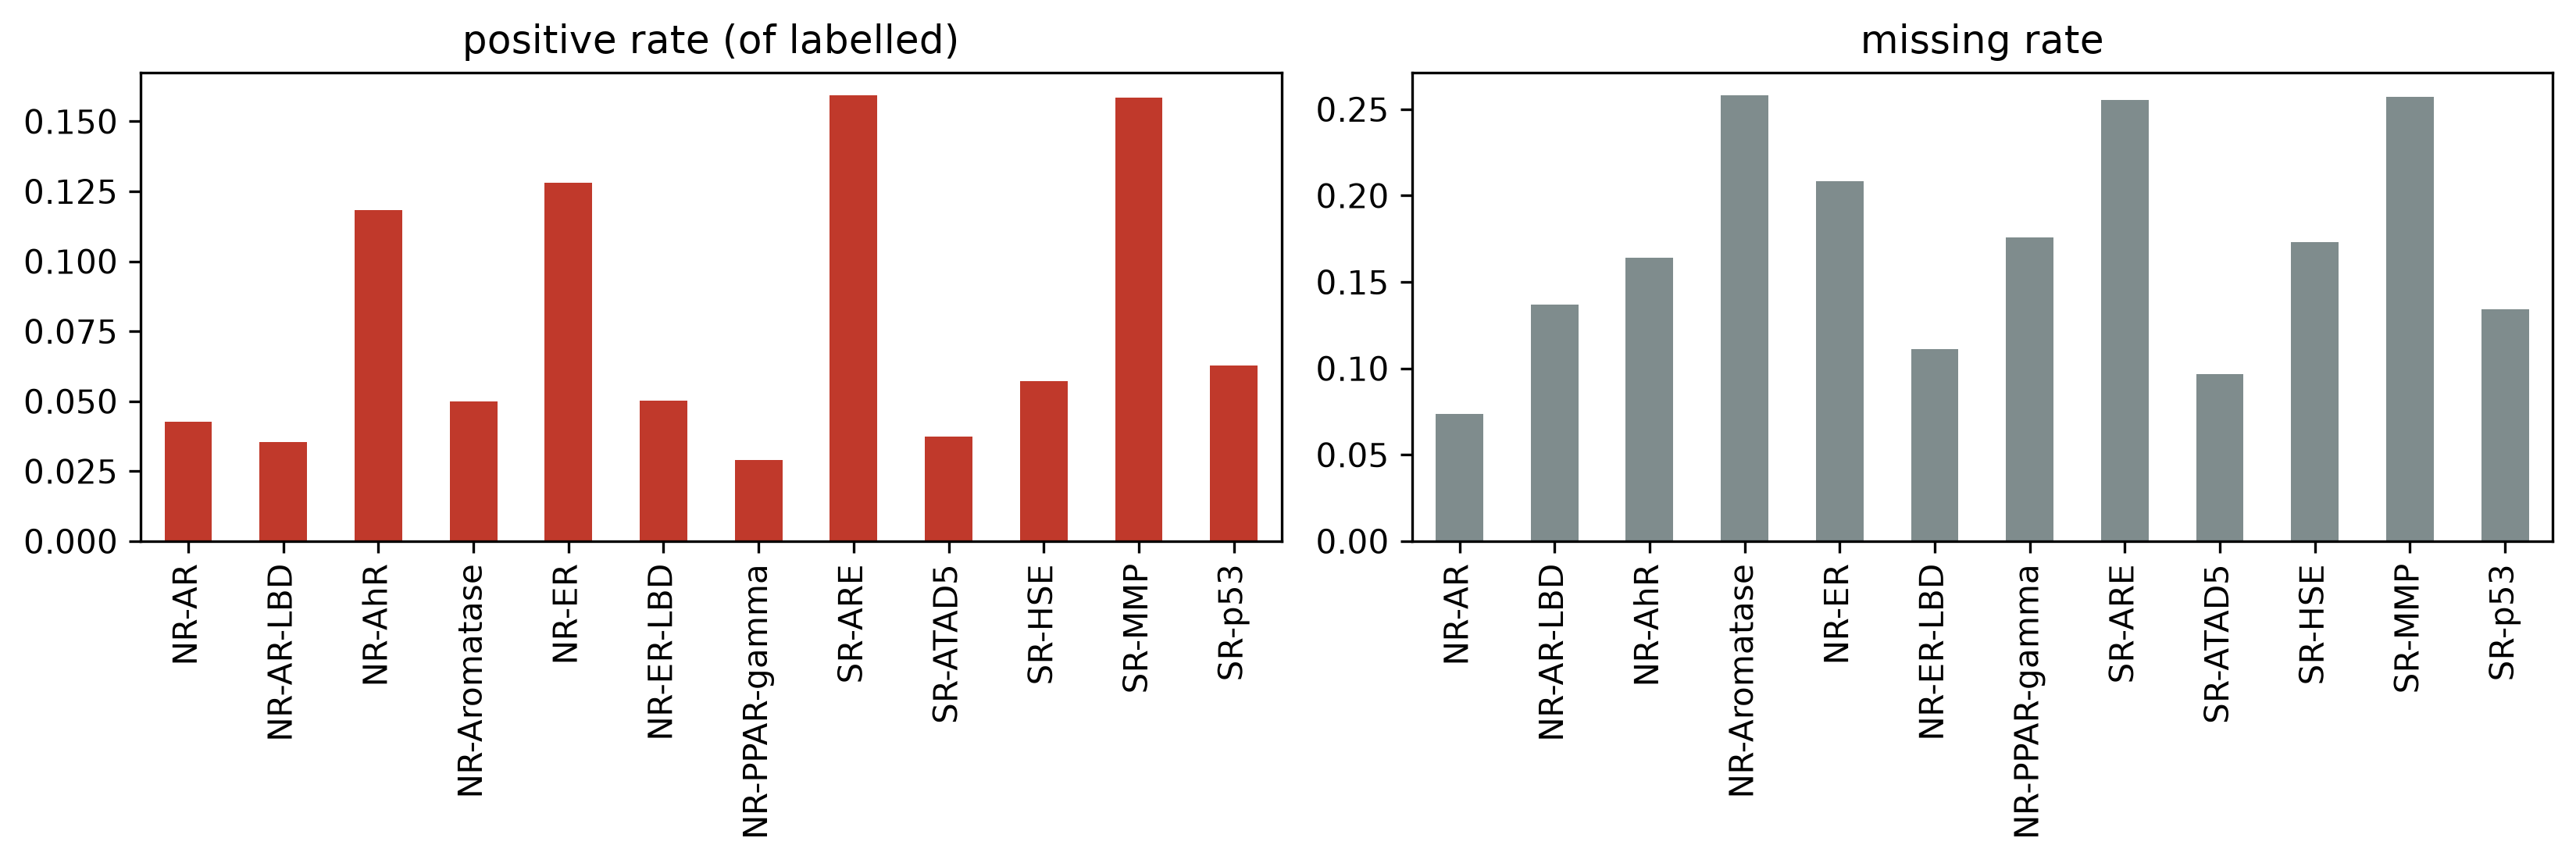
\includegraphics[width=\columnwidth]{eda_label_rates.png}
\caption{Positive rate (among labelled molecules) and missing rate per endpoint.}
\label{fig:labels}
\end{figure}

\section{Theoretical Background}
\label{sec:theory}

\subsection{Why scaffold splits}
The Bemis--Murcko scaffold~\cite{bemis1996murcko} of a molecule is what remains after removing all side chains: its ring systems and the linkers between them. Molecules sharing a scaffold are usually close analogues with correlated activity. Under a random split, a test molecule almost always has a training molecule with the same scaffold, so a model can score well by recognising near-duplicates. A scaffold split assigns whole scaffold groups to one part, so every test scaffold is unseen during training. That is closer to the prospective use case (screening a new chemical series); MoleculeNet uses it for several of its benchmarks~\cite{wu2018moleculenet}, and Yang et al.~\cite{yang2019analyzing} showed that random splits overstate performance for all model families. The difference between random and scaffold performance is our measure of the \emph{generalization penalty}.

\subsection{ROC-AUC versus PR-AUC under imbalance}
ROC-AUC equals the probability that a random positive is scored above a random negative,
\begin{equation}
\text{ROC-AUC} = P\big(s(x^+) > s(x^-)\big),
\end{equation}
which does not depend on the class ratio; a random classifier gets 0.5. Precision, $\mathrm{TP}/(\mathrm{TP}+\mathrm{FP})$, does depend on it: with a positive rate $\pi = 0.03$ there are about 32 negatives per positive, so even a small false-positive \emph{rate} gives many false positives and low precision. We report PR-AUC as average precision,
\begin{equation}
\text{AP} = \sum_n (R_n - R_{n-1})\, P_n,
\end{equation}
whose value for a random classifier is $\pi$, not 0.5~\cite{saito2015prc}. PR-AUC is therefore always reported next to the positive rate of that test set, and PR-AUC is only compared between models on the same split.

\subsection{Class weighting}
With few positives, the unweighted log-loss is dominated by negatives. Balanced class weights scale each example's loss by $w_c = n / (2 n_c)$, which makes both classes contribute equally to the loss. For XGBoost, \texttt{scale\_pos\_weight} $= n_\text{neg}/n_\text{pos}$ multiplies the gradient and Hessian of every positive by the same factor~\cite{chen2016xgboost}. Reweighting changes where the model spends capacity and shifts its probabilities upwards (they are no longer calibrated), but the ranking metrics we report are unaffected by calibration. All weights are computed on the training part only.

\subsection{Missing labels and leakage}
Each endpoint's model is trained only on rows where that endpoint is labelled, and the scorer drops unlabelled rows per task. Filling missing labels with 0 would inject false negatives at a rate far above the true positive rate. Two further leakage sources are closed off: duplicates are merged \emph{before} splitting (otherwise the same compound can sit in train and test), and every fitted preprocessing step (imputer, scaler, variance filter, class weights) sees training rows only.

\section{Methods}
\subsection{Splits}
We produce seven 80/10/10 splits keyed by canonical SMILES:
\texttt{scaffold\_det} follows the DeepChem convention, filling train with the largest scaffold groups first, then validation, then test; this is the number comparable to the literature. \texttt{scaffold\_s\{0,1,2\}} are balanced random scaffold splits: groups larger than half the test size go to train and the remaining groups are shuffled by seed, giving seed variance on the hard split. \texttt{random\_s\{0,1,2\}} split molecules uniformly at random and are used only to measure the scaffold gap. Tests check that the parts are disjoint, cover the dataset, and share no scaffold. Every task has at least one positive in each validation and test part.

\subsection{Features}
\textbf{Morgan fingerprints}~\cite{rogers2010ecfp} with radius 2 and 2048 bits. A molecule sets 30 bits on average (density 1.5\%); all 2048 bits are used somewhere, but 1{,}487 are set in fewer than 1\% of molecules. The dataset contains 26{,}749 distinct radius-$\le$2 environments, so after folding \emph{every} bit is shared by several substructures (13 on average at 2048 bits, 26 at 1024). A single bit's importance therefore cannot be read as one substructure.

\textbf{RDKit descriptors}: all 217 2D descriptors. \texttt{Ipc} reaches $10^{41}$, which overflows the float32 inputs of the tree models, so it is replaced by $\log(1+\texttt{Ipc})$. Twelve charge and BCUT descriptors are undefined for 107 molecules, 100 of which contain a metal or metalloid. The descriptor pipeline maps $\pm\infty$ to missing, imputes the training median, drops columns that are constant on train, and standardizes. It is a single scikit-learn \texttt{Pipeline} fitted on training rows only. The FP+desc feature set concatenates the raw bits with the processed descriptors.

\subsection{Models and tuning}
One model is trained per endpoint for each of six configurations: \{logistic regression, random forest~\cite{breiman2001rf}, XGBoost~\cite{chen2016xgboost}\} $\times$ \{FP, FP+descriptors\}. Logistic regression uses liblinear with $C \in \{0.01, 0.1, 1\}$ and balanced class weights. Random forest uses 500 trees, $\sqrt{d}$ features per split, \texttt{min\_samples\_leaf} $\in \{1, 3\}$ and balanced-subsample weights. XGBoost uses up to 1000 trees, learning rate 0.05, depth $\in \{4, 6\}$, row subsample 0.8, column subsample 0.5, and early stopping (patience 50) on validation PR-AUC. For each endpoint, the grid point with the highest \emph{validation} PR-AUC is kept, and the configuration used for our headline claims is also chosen on validation. The test set is scored once, at the end, by a single shared scorer.

\texttt{scaffold\_det} is run with three model seeds; each randomized split is run with its own seed. Every table therefore reports mean $\pm$ standard deviation over three runs. Logistic regression with liblinear is deterministic, so its standard deviation on \texttt{scaffold\_det} is zero.

\section{Results}
All numbers below are test-set means over 12 endpoints, reported as mean $\pm$ standard deviation over three runs, and come from \texttt{results/headline.csv}. Missing labels are excluded per endpoint.

\begin{table*}[t]
\centering
\caption{Test ROC-AUC and PR-AUC (12-endpoint mean, mean $\pm$ std over 3 runs). Mean test positive rate is 0.103 on both scaffold families and 0.077 on random, which is the PR-AUC of a random classifier.}
\label{tab:main}
\begin{tabular}{lcccccc}
\toprule
 & \multicolumn{3}{c}{ROC-AUC} & \multicolumn{3}{c}{PR-AUC} \\
\cmidrule(lr){2-4}\cmidrule(lr){5-7}
Model / features & scaffold\_det & scaffold & random & scaffold\_det & scaffold & random \\
\midrule
LR / FP & 0.715$\pm$0.000 & 0.775$\pm$0.036 & 0.801$\pm$0.013 & 0.319$\pm$0.000 & 0.395$\pm$0.051 & 0.435$\pm$0.038 \\
LR / FP+desc & 0.722$\pm$0.000 & 0.788$\pm$0.039 & 0.826$\pm$0.010 & 0.299$\pm$0.000 & 0.367$\pm$0.068 & 0.463$\pm$0.029 \\
RF / FP & 0.732$\pm$0.001 & 0.803$\pm$0.019 & 0.833$\pm$0.009 & 0.366$\pm$0.001 & 0.442$\pm$0.043 & 0.484$\pm$0.019 \\
RF / FP+desc & 0.782$\pm$0.003 & 0.839$\pm$0.024 & 0.862$\pm$0.002 & 0.406$\pm$0.002 & 0.481$\pm$0.043 & 0.531$\pm$0.016 \\
XGB / FP & 0.696$\pm$0.003 & 0.767$\pm$0.045 & 0.801$\pm$0.012 & 0.306$\pm$0.006 & 0.389$\pm$0.047 & 0.435$\pm$0.024 \\
XGB / FP+desc & 0.761$\pm$0.008 & 0.813$\pm$0.032 & 0.855$\pm$0.007 & 0.391$\pm$0.008 & 0.446$\pm$0.057 & 0.520$\pm$0.020 \\
\bottomrule
\end{tabular}
\end{table*}

\textbf{Model selection.} On validation PR-AUC, the random forest with FP+desc is selected on \texttt{scaffold\_det} (0.451), and XGBoost with FP+desc is selected on the balanced scaffold (0.490) and random (0.542) families. The selected models reach test ROC-AUC $0.782\pm0.003$, $0.813\pm0.032$ and $0.855\pm0.007$ respectively. On test, the random forest is actually best on all three families, but we report the validation choice because choosing on test would be selection on the test set.

\textbf{Scaffold generalization gap.} Every configuration loses performance on unseen scaffolds (Table~\ref{tab:main}, Fig.~\ref{fig:gap}). Going from random to \texttt{scaffold\_det}, ROC-AUC drops by 0.080 (RF, FP+desc) to 0.105 (XGB, FP). The balanced scaffold splits lie in between and vary far more between seeds (ROC-AUC std 0.02--0.05 vs.\ below 0.01 on \texttt{scaffold\_det}), because the split itself changes. A single deterministic scaffold split hides that variance. PR-AUC should be compared only within a column, since the test positive rate differs between split families.

\textbf{Features.} Adding descriptors to fingerprints improves validation PR-AUC on all 12 endpoints for XGBoost and 8/12 for random forests, but only 5/12 for logistic regression. The fingerprint ablation (Table~\ref{tab:abl}) shows that radius and length hardly matter on \texttt{scaffold\_det}, and that descriptors alone equal the combined set for XGBoost (ROC-AUC 0.761 both). Descriptors make up under 10\% of the columns but account for 34--57\% of XGBoost's total gain, with chemically sensible top features: aromatic ring counts for NR-AhR (whose ligands are planar aromatics) and phenol counts for SR-MMP.

\begin{table}[t]
\centering
\caption{Fingerprint ablation, XGBoost on \texttt{scaffold\_det}, test mean $\pm$ std over 3 seeds.}
\label{tab:abl}
\begin{tabular}{lcc}
\toprule
Features & ROC-AUC & PR-AUC \\
\midrule
Morgan r1, 1024 bits & 0.704$\pm$0.003 & 0.323$\pm$0.012 \\
Morgan r1, 2048 bits & 0.693$\pm$0.006 & 0.303$\pm$0.006 \\
Morgan r2, 1024 bits & 0.688$\pm$0.002 & 0.297$\pm$0.007 \\
Morgan r2, 2048 bits & 0.696$\pm$0.003 & 0.306$\pm$0.006 \\
Morgan r3, 1024 bits & 0.683$\pm$0.007 & 0.300$\pm$0.010 \\
Morgan r3, 2048 bits & 0.695$\pm$0.008 & 0.304$\pm$0.005 \\
descriptors only & 0.761$\pm$0.001 & 0.402$\pm$0.003 \\
\bottomrule
\end{tabular}
\end{table}

\begin{figure}[t]
\centering
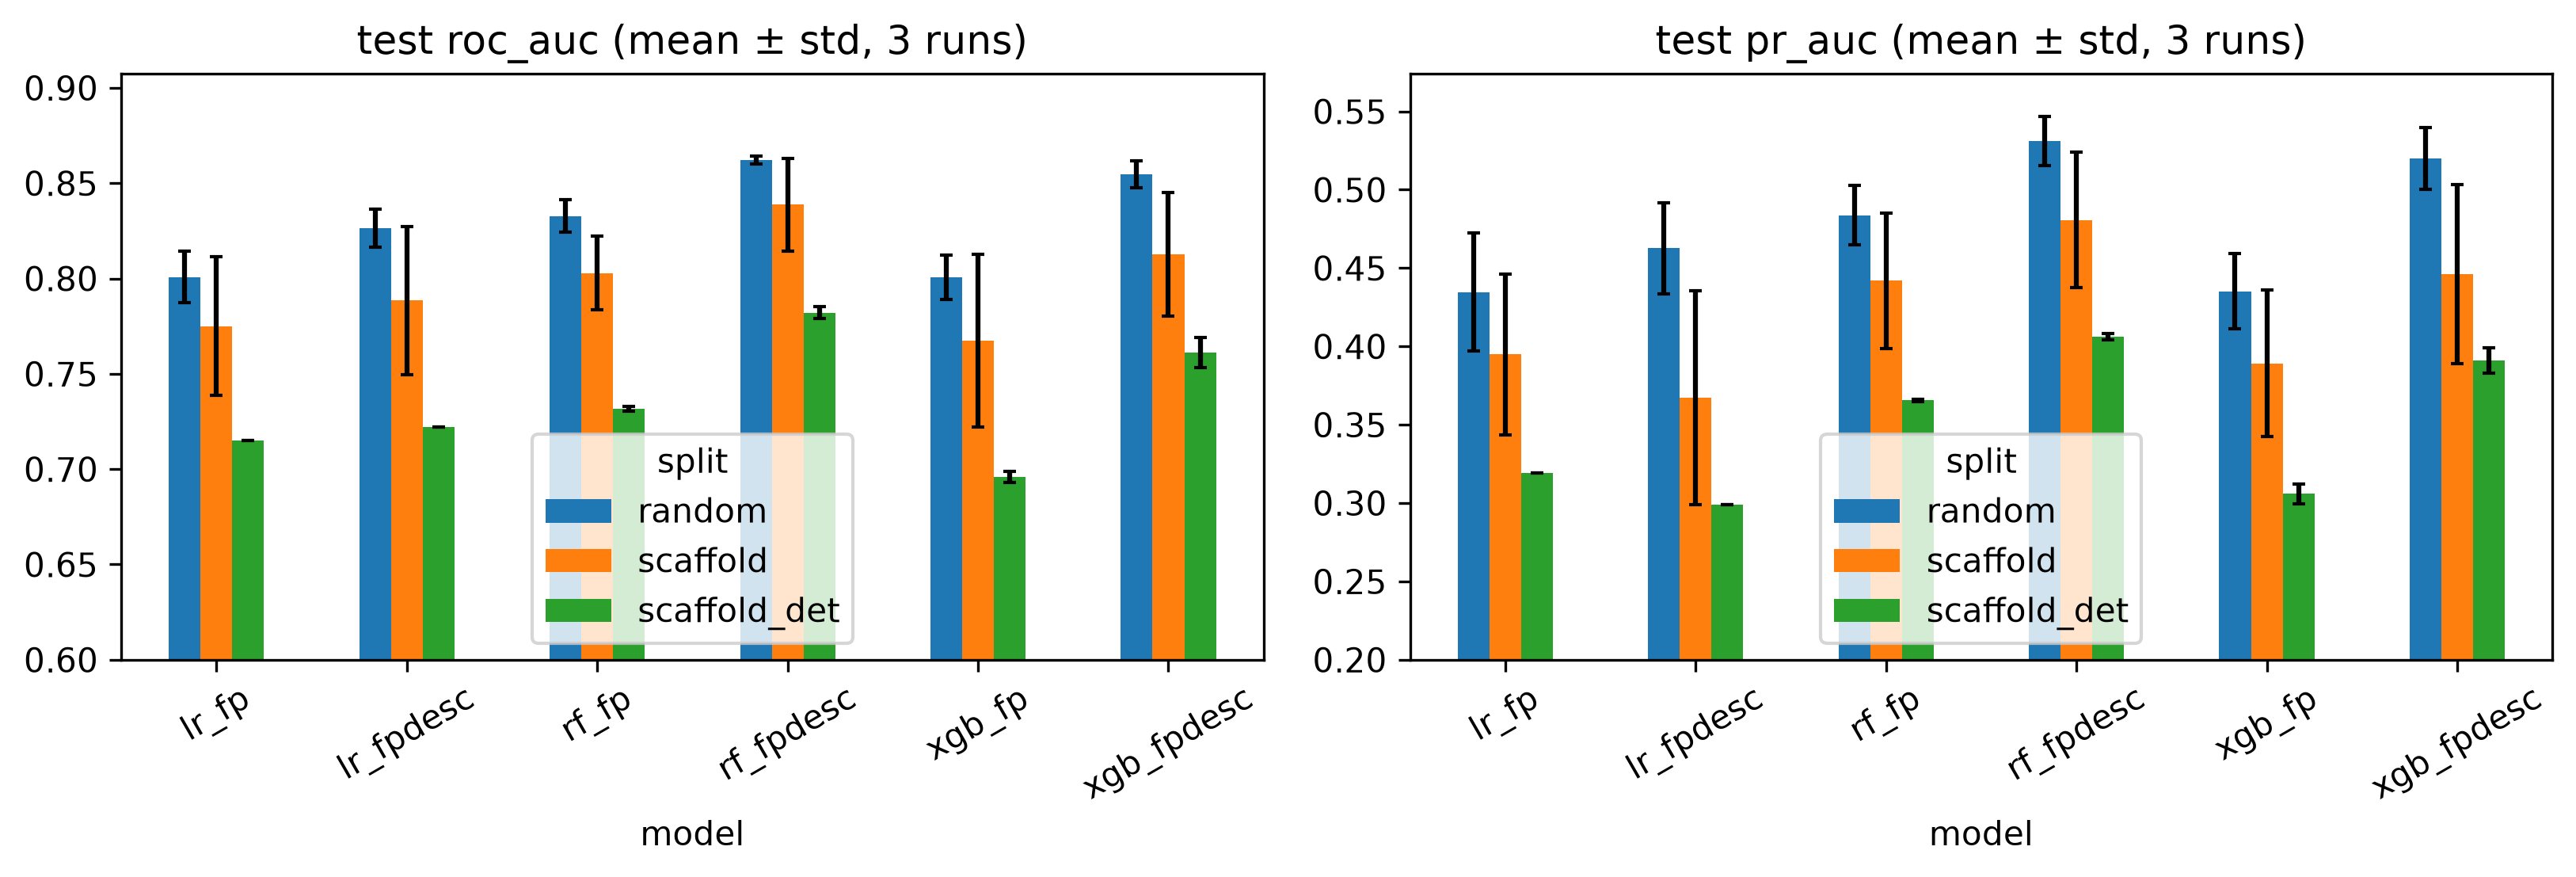
\includegraphics[width=\columnwidth]{aml_test_split_gap.png}
\caption{Test ROC-AUC and PR-AUC by split family; error bars are std over 3 runs.}
\label{fig:gap}
\end{figure}

\textbf{Per endpoint.} For the selected random forest on \texttt{scaffold\_det}, ROC-AUC ranges from 0.692 (NR-ER) to 0.866 (SR-MMP). The weakest PR-AUC is SR-ATAD5 (0.229, at a positive rate of 0.051), which is still 4.5$\times$ its random baseline.

\section{Limitations}
Tox21 assays are in-vitro screens of pathway activity, not measurements of whole-organism toxicity. The labels are noisy: we found conflicting duplicate measurements, and some endpoints have only a few hundred positives, so per-endpoint scores on a 770-molecule test set move noticeably between seeds. A scaffold split is harder than a random one, but it is still a retrospective split of one dataset rather than true prospective validation. Finally, stereochemistry and charges were kept as given, so stereoisomers count as separate molecules; this is a deliberate choice but a different convention would change the duplicate counts slightly.

The validation set is reused. Every configuration picks its hyper-parameters on it, the reported model is chosen on it, and XGBoost also uses it for early stopping, so validation scores (XGBoost's especially) are optimistic. With few validation positives the early-stopping signal is noisy: 33 of the 216 XGBoost endpoint fits keep 20 trees or fewer (as few as 2, at learning rate 0.05). This may explain why validation selects XGBoost on the balanced scaffold and random families while the random forest is best on test. The test set takes no part in any of these choices, so the reported test numbers are unaffected.

\section{Conclusion}
A carefully deduplicated, leakage-controlled classical pipeline gives a test ROC-AUC of 0.78 on the deterministic scaffold split, against 0.86 for the same model on random splits. The scaffold gap (0.08--0.11 ROC-AUC) is as large as the spread between the worst and best classical configuration on the same split (0.086), so the choice of evaluation split matters as much as the choice of model. On unseen scaffolds, whole-molecule descriptors carry most of the signal. Phase~2 tests whether learned graph representations shrink this gap, using the same splits, seeds and scorer so that the comparison is direct.

\bibliographystyle{IEEEtran}
\bibliography{references}

\end{document}
